% Options for packages loaded elsewhere
\PassOptionsToPackage{unicode}{hyperref}
\PassOptionsToPackage{hyphens}{url}
%
\documentclass[
]{book}
\usepackage{amsmath,amssymb}
\usepackage{iftex}
\ifPDFTeX
  \usepackage[T1]{fontenc}
  \usepackage[utf8]{inputenc}
  \usepackage{textcomp} % provide euro and other symbols
\else % if luatex or xetex
  \usepackage{unicode-math} % this also loads fontspec
  \defaultfontfeatures{Scale=MatchLowercase}
  \defaultfontfeatures[\rmfamily]{Ligatures=TeX,Scale=1}
\fi
\usepackage{lmodern}
\ifPDFTeX\else
  % xetex/luatex font selection
\fi
% Use upquote if available, for straight quotes in verbatim environments
\IfFileExists{upquote.sty}{\usepackage{upquote}}{}
\IfFileExists{microtype.sty}{% use microtype if available
  \usepackage[]{microtype}
  \UseMicrotypeSet[protrusion]{basicmath} % disable protrusion for tt fonts
}{}
\makeatletter
\@ifundefined{KOMAClassName}{% if non-KOMA class
  \IfFileExists{parskip.sty}{%
    \usepackage{parskip}
  }{% else
    \setlength{\parindent}{0pt}
    \setlength{\parskip}{6pt plus 2pt minus 1pt}}
}{% if KOMA class
  \KOMAoptions{parskip=half}}
\makeatother
\usepackage{xcolor}
\usepackage{color}
\usepackage{fancyvrb}
\newcommand{\VerbBar}{|}
\newcommand{\VERB}{\Verb[commandchars=\\\{\}]}
\DefineVerbatimEnvironment{Highlighting}{Verbatim}{commandchars=\\\{\}}
% Add ',fontsize=\small' for more characters per line
\usepackage{framed}
\definecolor{shadecolor}{RGB}{248,248,248}
\newenvironment{Shaded}{\begin{snugshade}}{\end{snugshade}}
\newcommand{\AlertTok}[1]{\textcolor[rgb]{0.94,0.16,0.16}{#1}}
\newcommand{\AnnotationTok}[1]{\textcolor[rgb]{0.56,0.35,0.01}{\textbf{\textit{#1}}}}
\newcommand{\AttributeTok}[1]{\textcolor[rgb]{0.13,0.29,0.53}{#1}}
\newcommand{\BaseNTok}[1]{\textcolor[rgb]{0.00,0.00,0.81}{#1}}
\newcommand{\BuiltInTok}[1]{#1}
\newcommand{\CharTok}[1]{\textcolor[rgb]{0.31,0.60,0.02}{#1}}
\newcommand{\CommentTok}[1]{\textcolor[rgb]{0.56,0.35,0.01}{\textit{#1}}}
\newcommand{\CommentVarTok}[1]{\textcolor[rgb]{0.56,0.35,0.01}{\textbf{\textit{#1}}}}
\newcommand{\ConstantTok}[1]{\textcolor[rgb]{0.56,0.35,0.01}{#1}}
\newcommand{\ControlFlowTok}[1]{\textcolor[rgb]{0.13,0.29,0.53}{\textbf{#1}}}
\newcommand{\DataTypeTok}[1]{\textcolor[rgb]{0.13,0.29,0.53}{#1}}
\newcommand{\DecValTok}[1]{\textcolor[rgb]{0.00,0.00,0.81}{#1}}
\newcommand{\DocumentationTok}[1]{\textcolor[rgb]{0.56,0.35,0.01}{\textbf{\textit{#1}}}}
\newcommand{\ErrorTok}[1]{\textcolor[rgb]{0.64,0.00,0.00}{\textbf{#1}}}
\newcommand{\ExtensionTok}[1]{#1}
\newcommand{\FloatTok}[1]{\textcolor[rgb]{0.00,0.00,0.81}{#1}}
\newcommand{\FunctionTok}[1]{\textcolor[rgb]{0.13,0.29,0.53}{\textbf{#1}}}
\newcommand{\ImportTok}[1]{#1}
\newcommand{\InformationTok}[1]{\textcolor[rgb]{0.56,0.35,0.01}{\textbf{\textit{#1}}}}
\newcommand{\KeywordTok}[1]{\textcolor[rgb]{0.13,0.29,0.53}{\textbf{#1}}}
\newcommand{\NormalTok}[1]{#1}
\newcommand{\OperatorTok}[1]{\textcolor[rgb]{0.81,0.36,0.00}{\textbf{#1}}}
\newcommand{\OtherTok}[1]{\textcolor[rgb]{0.56,0.35,0.01}{#1}}
\newcommand{\PreprocessorTok}[1]{\textcolor[rgb]{0.56,0.35,0.01}{\textit{#1}}}
\newcommand{\RegionMarkerTok}[1]{#1}
\newcommand{\SpecialCharTok}[1]{\textcolor[rgb]{0.81,0.36,0.00}{\textbf{#1}}}
\newcommand{\SpecialStringTok}[1]{\textcolor[rgb]{0.31,0.60,0.02}{#1}}
\newcommand{\StringTok}[1]{\textcolor[rgb]{0.31,0.60,0.02}{#1}}
\newcommand{\VariableTok}[1]{\textcolor[rgb]{0.00,0.00,0.00}{#1}}
\newcommand{\VerbatimStringTok}[1]{\textcolor[rgb]{0.31,0.60,0.02}{#1}}
\newcommand{\WarningTok}[1]{\textcolor[rgb]{0.56,0.35,0.01}{\textbf{\textit{#1}}}}
\usepackage{longtable,booktabs,array}
\usepackage{calc} % for calculating minipage widths
% Correct order of tables after \paragraph or \subparagraph
\usepackage{etoolbox}
\makeatletter
\patchcmd\longtable{\par}{\if@noskipsec\mbox{}\fi\par}{}{}
\makeatother
% Allow footnotes in longtable head/foot
\IfFileExists{footnotehyper.sty}{\usepackage{footnotehyper}}{\usepackage{footnote}}
\makesavenoteenv{longtable}
\usepackage{graphicx}
\makeatletter
\newsavebox\pandoc@box
\newcommand*\pandocbounded[1]{% scales image to fit in text height/width
  \sbox\pandoc@box{#1}%
  \Gscale@div\@tempa{\textheight}{\dimexpr\ht\pandoc@box+\dp\pandoc@box\relax}%
  \Gscale@div\@tempb{\linewidth}{\wd\pandoc@box}%
  \ifdim\@tempb\p@<\@tempa\p@\let\@tempa\@tempb\fi% select the smaller of both
  \ifdim\@tempa\p@<\p@\scalebox{\@tempa}{\usebox\pandoc@box}%
  \else\usebox{\pandoc@box}%
  \fi%
}
% Set default figure placement to htbp
\def\fps@figure{htbp}
\makeatother
\setlength{\emergencystretch}{3em} % prevent overfull lines
\providecommand{\tightlist}{%
  \setlength{\itemsep}{0pt}\setlength{\parskip}{0pt}}
\setcounter{secnumdepth}{5}
\usepackage{booktabs}
\usepackage{amsthm}
\makeatletter
\def\thm@space@setup{%
  \thm@preskip=8pt plus 2pt minus 4pt
  \thm@postskip=\thm@preskip
}
\makeatother
\usepackage[]{natbib}
\bibliographystyle{apalike}
\usepackage{bookmark}
\IfFileExists{xurl.sty}{\usepackage{xurl}}{} % add URL line breaks if available
\urlstyle{same}
\hypersetup{
  pdftitle={Estadística Multivariada},
  pdfauthor={Haydeé Peruyero},
  hidelinks,
  pdfcreator={LaTeX via pandoc}}

\title{Estadística Multivariada}
\author{Haydeé Peruyero}
\date{}

\begin{document}
\maketitle

{
\setcounter{tocdepth}{1}
\tableofcontents
}
\chapter{Estadística Multivariada}\label{estaduxedstica-multivariada}

\section{Temario}\label{temario}

\begin{enumerate}
\def\labelenumi{\arabic{enumi}.}
\tightlist
\item
  Regresión múltiple
\end{enumerate}

1.1 Mínimos cuadrados.

1.2 Medidas de bondad de ajuste.

1.3 Determinación del número de variables predictorias.

\begin{enumerate}
\def\labelenumi{\arabic{enumi}.}
\setcounter{enumi}{1}
\tightlist
\item
  Análisis de componentes principales
\end{enumerate}

2.1 Descripción de la metodología.

2.2 Técnicas de extracción de componentes principales.

2.3 Determinación del número de componentes principales.

\begin{enumerate}
\def\labelenumi{\arabic{enumi}.}
\setcounter{enumi}{2}
\tightlist
\item
  Análisis factorial
\end{enumerate}

3.1 Descripción de la metodología del análisis factorial.

3.2 Descripción del modelo básico.

3.3 Método de cálculo.

3.4 Comparación con la técnica del análisis de componentes principales.

3.5 Usos de software (R, Minitab, SciPy, entre otros).

\begin{enumerate}
\def\labelenumi{\arabic{enumi}.}
\setcounter{enumi}{3}
\tightlist
\item
  Análisis de conglomerados
\end{enumerate}

4.1Descripción de la metodología de análisis de conglomerados.

4.2 Técnicas de jerarquización y de particionamiento.

4.3 Implementación computacional.

4.4 Usos de los dendogramas.

4.5 Usos de software (R, Minitab, SciPy, entre otros).

\begin{enumerate}
\def\labelenumi{\arabic{enumi}.}
\setcounter{enumi}{4}
\tightlist
\item
  Análisis discriminante
\end{enumerate}

5.1 Descripción de la metodología del análisis discriminante.

5.2 Discriminación entre dos grupos.

5.3 Contribución por variable.

5.4 Discriminación logística.

5.5 Discriminación múltiple.

5.6 Usos de software (R, Minitab, SciPy, entre otros).

A1. R

A2. Git + Github

A3. Gráficas Multivariadas

A4. Escalas de Medición

A5. Valores Faltantes

\section{Evaluación}\label{evaluaciuxf3n}

\begin{itemize}
\tightlist
\item
  Examenes 50\%
\item
  Tareas 25\%
\item
  Proyecto 20\%
\item
  DataCamp 5\%
\end{itemize}

\section{Proyecto final}\label{proyecto-final}

\begin{itemize}
\tightlist
\item
  Buscar una base de datos ``real''
\item
  Aplicar 3 métodos de estadística multivariada
\item
  Entregar documento con:

  \begin{itemize}
  \tightlist
  \item
    Descripción de los datos
  \item
    Planteamiento del problema
  \item
    Métodos usados
  \item
    Interpretación de resultados
  \item
    Código usado
  \end{itemize}
\item
  Repositorio con código reproducible
\item
  Exposición de resultados
\end{itemize}

\section{Referencias}\label{referencias}

{[}1{]}

\section{Material interesante}\label{material-interesante}

\begin{itemize}
\tightlist
\item
  \href{https://bookdown.org/}{Bookdown}.
\item
  \href{https://swcarpentry.github.io/r-novice-gapminder/}{Software Carpentry}.
\item
  \href{https://swcarpentry.github.io/git-novice/14-supplemental-rstudio/}{Git}
\item
  \href{https://info5940.infosci.cornell.edu/setup/git/what-is-git/}{Why Git}
\item
  \href{https://bookdown.org/yihui/rmarkdown-cookbook/}{R Markdown Cookbook}
\item
  \href{http://www.sthda.com/english/wiki/data-visualization}{STHDA}
\item
  \href{https://bookdown.org/ndphillips/YaRrr/}{YaRrr! The Pirate's Guide to R}
\item
  \href{https://link.springer.com/book/10.1007/978-3-319-53019-2}{Learn ggplot2 Using Shiny App}
\item
  \href{https://link.springer.com/book/10.1007/978-0-387-98141-3}{Ggplot2: Elegant Graphics for Data Analysis}

  \begin{itemize}
  \tightlist
  \item
    \href{https://ggplot2-book.org/index.html}{Versión online}
  \end{itemize}
\item
  \href{https://www.springer.com/series/6991/books}{Use R! Colección Springer}
\item
  \href{https://link.springer.com/book/10.1007/978-0-387-75969-2}{Lattice: Multivariate Data Visualization with R}
\item
  \href{http://www.cookbook-r.com/}{R Graphics cookbook}
\item
  \href{https://education.github.com/benefits}{Cuenta pro de Github}
\end{itemize}

\section{DataCamp}\label{datacamp}

\begin{figure}
\centering
\pandocbounded{
\includegraphics[keepaspectratio]{img/regular.png}}
\caption{DataCamp}
\end{figure}

\chapter{Regresión múltiple}\label{regresiuxf3n-muxfaltiple}

\section{¿Por qué estadística multivariada?}\label{por-quuxe9-estaduxedstica-multivariada}

El proceso de modelado consiste en construir expresiones matemáticas que permitan representar el comportamiento de una variable que queremos estudiar. Cuando contamos con varias variables, suele interesarnos analizar cómo unas influyen sobre otras, determinando si existe una relación, su intensidad y su forma. En muchos casos, estas relaciones pueden ser complejas y difíciles de describir directamente; por ello, se busca aproximarlas mediante funciones matemáticas sencillas como polinomios, que conserven los elementos esenciales para explicar el fenómeno de interés.

Cuando estudiamos fenómenos deterministas, es común vincular una variable dependiente con una o más variables independientes. Por ejemplo, en la ecuación de la velocidad (\(v=d/t\)), la distancia depende de la velocidad y del tiempo. En la práctica, cuando realizamos distintos experimentos, las fórmulas deterministas podrían no capturar por completo el comportamiento observado. Esto puede deberse a factores no controlados, a la presencia de variabilidad natural o a efectos aleatorios. Por esta razón, además de la parte determinista del modelo, se incorpora un término que represente la discrepancia aleatoria entre lo que se predice y lo que efectivamente se observa. De forma general, esta idea se resume como:

\[Observación = Modelo \ + \ Error\]

Cuando se supone que la relación entre las variables puede representarse mediante una ecuación lineal, hablamos de \emph{análisis de regresión lineal}. Si intervienen únicamente dos variables, una dependiente \(y\) y independiente \(x\), se trata de \textbf{regresión lineal simple}. En cambio, cuando la variable de interés \(y\) depende de dos o más variables independientes \(x_1,x_2, ...\) hablamos de \textbf{regresión lineal múltiple}.

\emph{Supongamos que queremos predecir el rendimiento académico de un estudiante, ¿solo necesitamos las horas que estudia?}

En este caso se tiene que el puntaje o rendimiento lo podemos representar con \(y\) y las horas de estudio con \(x\). Entonces esta propuesta de modelo, la podríamos representar como:

\[y=\beta_0+\beta_1x\]
Donde \(\beta_0\) es la ordenada al origen y \(\beta_1\) la pendiente. Esta recta podría no ajustarse al modelo por diferentes razones, entonces lo que se hace es considerar un error aleatorio \(\epsilon\). El modelo que ya considera este error se representa como:

\[y=\beta_0+\beta_1x+\epsilon.\]

A este modelo se le conoce como modelo de \textbf{regresión lineal simple} y a \(\beta_0,\beta_1\) se les conoce como \textbf{coeficientes de regresión}.

En problemas reales, casi nunca una sola variable explica el fenómeno. Las decisiones y predicciones mejoran cuando integramos múltiples fuentes de información.

Ejemplos:
- Salud: riesgo de una enfermedad según edad, IMC, actividad física, dieta y antecedentes.
- Ingeniería: vida útil de una pieza según temperatura, vibración, material y carga.
- Biología: crecimiento de una planta por agua, luz, fertilizante, temperatura.

\textbf{Ejemplo:} Si queremos predecir el rendimiento académico de un estudiante, ¿solo necesitamos las horas que estudia? ¿qué otras variables podrían influir en el puntaje de un examen?

Rendimiento escolar

\begin{Shaded}
\begin{Highlighting}[]
\FunctionTok{set.seed}\NormalTok{(}\DecValTok{123}\NormalTok{)}
\NormalTok{n }\OtherTok{\textless{}{-}} \DecValTok{10}
\NormalTok{data\_intro }\OtherTok{\textless{}{-}} \FunctionTok{tibble}\NormalTok{(}
  \AttributeTok{estudiante =} \FunctionTok{paste0}\NormalTok{(}\StringTok{"E"}\NormalTok{, }\DecValTok{1}\SpecialCharTok{:}\NormalTok{n),}
  \AttributeTok{horas\_estudio =} \FunctionTok{c}\NormalTok{(}\DecValTok{2}\NormalTok{,}\DecValTok{3}\NormalTok{,}\DecValTok{4}\NormalTok{,}\DecValTok{5}\NormalTok{,}\DecValTok{1}\NormalTok{,}\DecValTok{3}\NormalTok{,}\DecValTok{2}\NormalTok{,}\DecValTok{4}\NormalTok{,}\DecValTok{5}\NormalTok{,}\DecValTok{6}\NormalTok{),}
  \AttributeTok{horas\_sueno  =} \FunctionTok{c}\NormalTok{(}\DecValTok{7}\NormalTok{,}\DecValTok{8}\NormalTok{,}\DecValTok{6}\NormalTok{,}\DecValTok{7}\NormalTok{,}\DecValTok{5}\NormalTok{,}\DecValTok{8}\NormalTok{,}\DecValTok{7}\NormalTok{,}\DecValTok{6}\NormalTok{,}\DecValTok{9}\NormalTok{,}\DecValTok{7}\NormalTok{),}
  \AttributeTok{asistencia   =} \FunctionTok{c}\NormalTok{(}\FloatTok{0.9}\NormalTok{,}\FloatTok{0.95}\NormalTok{,}\FloatTok{0.8}\NormalTok{,}\FloatTok{0.85}\NormalTok{,}\FloatTok{0.7}\NormalTok{,}\FloatTok{0.9}\NormalTok{,}\FloatTok{0.8}\NormalTok{,}\FloatTok{0.9}\NormalTok{,}\DecValTok{1}\NormalTok{,}\FloatTok{0.95}\NormalTok{),}
  \AttributeTok{puntaje      =} \FunctionTok{c}\NormalTok{(}\DecValTok{65}\NormalTok{,}\DecValTok{70}\NormalTok{,}\DecValTok{68}\NormalTok{,}\DecValTok{80}\NormalTok{,}\DecValTok{60}\NormalTok{,}\DecValTok{75}\NormalTok{,}\DecValTok{65}\NormalTok{,}\DecValTok{78}\NormalTok{,}\DecValTok{88}\NormalTok{,}\DecValTok{85}\NormalTok{)}
\NormalTok{)}
\NormalTok{data\_intro}
\end{Highlighting}
\end{Shaded}

\begin{verbatim}
## # A tibble: 10 x 5
##    estudiante horas_estudio horas_sueno asistencia puntaje
##    <chr>              <dbl>       <dbl>      <dbl>   <dbl>
##  1 E1                     2           7       0.9       65
##  2 E2                     3           8       0.95      70
##  3 E3                     4           6       0.8       68
##  4 E4                     5           7       0.85      80
##  5 E5                     1           5       0.7       60
##  6 E6                     3           8       0.9       75
##  7 E7                     2           7       0.8       65
##  8 E8                     4           6       0.9       78
##  9 E9                     5           9       1         88
## 10 E10                    6           7       0.95      85
\end{verbatim}

¿Qué pasa si solo graficamos horas de estudio vs puntaje?

Plot hotas de estudio vs puntaje sugerida

\begin{Shaded}
\begin{Highlighting}[]
\FunctionTok{library}\NormalTok{(ggplot2)}
\FunctionTok{ggplot}\NormalTok{(data\_intro, }\FunctionTok{aes}\NormalTok{(horas\_estudio, puntaje)) }\SpecialCharTok{+}
  \FunctionTok{geom\_point}\NormalTok{(}\AttributeTok{size=}\DecValTok{3}\NormalTok{) }\SpecialCharTok{+}
  \FunctionTok{geom\_smooth}\NormalTok{(}\AttributeTok{method=}\StringTok{"lm"}\NormalTok{, }\AttributeTok{se=}\ConstantTok{FALSE}\NormalTok{) }\SpecialCharTok{+}
  \FunctionTok{labs}\NormalTok{(}\AttributeTok{title=}\StringTok{"¿Solo horas de estudio explican el puntaje?"}\NormalTok{)}
\end{Highlighting}
\end{Shaded}

\begin{verbatim}
## `geom_smooth()` using formula = 'y ~ x'
\end{verbatim}

\pandocbounded{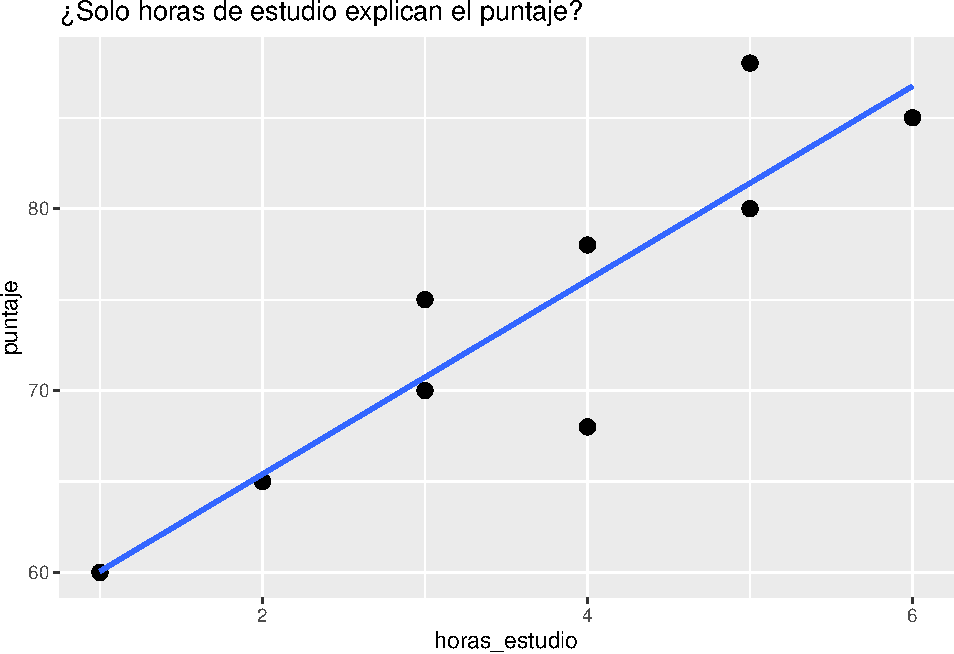
\includegraphics[keepaspectratio]{MultivariateStatisticalAnalysis_files/figure-latex/unnamed-chunk-3-1.pdf}}

¿Se ajusta un modelo lineal? ¿Porqué?

\subsection{¿Qué es ``multivariado'' y por qué lo necesitamos?}\label{quuxe9-es-multivariado-y-por-quuxe9-lo-necesitamos}

\textbf{Idea central:} cuando \textbf{varias} \(x\) influyen sobre \(y\), estudiar cada \(x\) por separado puede engañarnos. El análisis multivariado permite:

\begin{itemize}
\tightlist
\item
  \textbf{Aislar efectos}: estimar el efecto de \(x_1\) \emph{manteniendo constantes} \(x_2,x_3,...\).
\item
  \textbf{Mejorar predicción}: reducir error al añadir información relevante.
\item
  \textbf{Controlar confusores}: variables que cambian la relación aparente entre \(y\) y \(x\).
\end{itemize}

\textbf{Ejemplo:} Si ajustamos ahora un modelo con varias variables, ¿vamos a observar un cambio? ¿se ajustará mejor?

Código (modelos + comparaciones)

\begin{Shaded}
\begin{Highlighting}[]
\CommentTok{\# Modelo simple}
\NormalTok{m1 }\OtherTok{\textless{}{-}} \FunctionTok{lm}\NormalTok{(puntaje }\SpecialCharTok{\textasciitilde{}}\NormalTok{ horas\_estudio, }\AttributeTok{data =}\NormalTok{ data\_intro)}

\CommentTok{\# Modelo múltiple}
\NormalTok{m2 }\OtherTok{\textless{}{-}} \FunctionTok{lm}\NormalTok{(puntaje }\SpecialCharTok{\textasciitilde{}}\NormalTok{ horas\_estudio }\SpecialCharTok{+}\NormalTok{ horas\_sueno }\SpecialCharTok{+}\NormalTok{ asistencia, }\AttributeTok{data =}\NormalTok{ data\_intro)}

\CommentTok{\# Medidas clave}
\NormalTok{R2\_m1  }\OtherTok{\textless{}{-}} \FunctionTok{glance}\NormalTok{(m1)}\SpecialCharTok{$}\NormalTok{r.squared}
\NormalTok{R2\_m2  }\OtherTok{\textless{}{-}} \FunctionTok{glance}\NormalTok{(m2)}\SpecialCharTok{$}\NormalTok{r.squared}

\FunctionTok{print}\NormalTok{(}\FunctionTok{paste}\NormalTok{(}\StringTok{"El R2 del modelo simple:"}\NormalTok{, R2\_m1))}
\end{Highlighting}
\end{Shaded}

\begin{verbatim}
## [1] "El R2 del modelo simple: 0.824317362184441"
\end{verbatim}

\begin{Shaded}
\begin{Highlighting}[]
\FunctionTok{print}\NormalTok{(}\FunctionTok{paste}\NormalTok{(}\StringTok{"El R2 del modelo multiple:"}\NormalTok{, R2\_m2))}
\end{Highlighting}
\end{Shaded}

\begin{verbatim}
## [1] "El R2 del modelo multiple: 0.895428180549875"
\end{verbatim}

\begin{Shaded}
\begin{Highlighting}[]
\CommentTok{\#R2adj\_m1 \textless{}{-} glance(m1)$adj.r.squared}
\CommentTok{\#R2adj \_m2 \textless{}{-} glance(m2)$adj.r.squared}
\end{Highlighting}
\end{Shaded}

\begin{itemize}
\tightlist
\item
  ¿Aumentó \(R^2\) al incluir más variables? ¿Por qué tiende a subir?
\item
  ¿Qué cambia en la interpretación de horas\_estudio al controlar por horas\_sueno y asistencia?
\item
  ¿Puede un predictor ser importante en bivariado y no en multivariado (o viceversa)?
\end{itemize}

\section{Regresión múltiple}\label{regresiuxf3n-muxfaltiple-1}

\subsection{Modelo y estimación}\label{modelo-y-estimaciuxf3n}

Los modelos en regresión lineal múltiple están dados por la siguiente forma, donde \(y\) depende de \(p\) variables predictoras:

\[y_i=\beta_0+\beta_1x_{i1}+\beta_2x_{i2} + \beta_px_{ip}+\epsilon_i.\]

Se suele asumir que los errores \(\epsilon_i\) son i.i.d. con distribución normal de media 0 y varianza \(\sigma^2\) desconocida. Los coeficientes \(\beta_i\) son constantes desconocidas y son los parámetros del modelo. Cada \(\beta_j\) representa el cambio esperado en la respuesta \(y\) por el cambio unitario en \(x_i\) cuando todas las demás variables independientes \(x_i(i\neq j)\) se mantienen constantes.

\begin{Shaded}
\begin{Highlighting}[]
\CommentTok{\# Forma general}
\NormalTok{ajuste }\OtherTok{\textless{}{-}} \FunctionTok{lm}\NormalTok{(y }\SpecialCharTok{\textasciitilde{}}\NormalTok{ x1 }\SpecialCharTok{+}\NormalTok{ x2 }\SpecialCharTok{+}\NormalTok{ ... }\SpecialCharTok{+}\NormalTok{ xp, }\AttributeTok{data =}\NormalTok{ datos)}
\CommentTok{\# summary(ajuste)}
\end{Highlighting}
\end{Shaded}

Los coeficientes los podemos interpretar como sigue:

\begin{itemize}
\tightlist
\item
  \textbf{Intercepto (\(\beta_0\))}: valor esperado de \(y\) cuando todas las \(x\)=0.
\item
  \textbf{Pendiente \(\beta_j\)}: efecto \textbf{parcial} de \(x_j\) sobre \(y\) manteniendo las demás constantes.
\end{itemize}

En los modelos de regreción lineal, solemos usar las siguientes medidas de bondad de ajuste:

\begin{itemize}
\tightlist
\item
  \textbf{\(R^2\)}: proporción de varianza de \(y\) explicada.
\item
  \textbf{\(R^2\) ajustado}: penaliza por número de predictores (mejor para comparar modelos con distinto número de x).
\item
  \textbf{RMSE (\(\sigma\))}: error típico de predicción en unidades de \(y\).
\end{itemize}

\begin{Shaded}
\begin{Highlighting}[]
\NormalTok{comp }\OtherTok{\textless{}{-}}\NormalTok{ dplyr}\SpecialCharTok{::}\FunctionTok{bind\_rows}\NormalTok{(}
  \FunctionTok{glance}\NormalTok{(m1) }\SpecialCharTok{\%\textgreater{}\%} \FunctionTok{mutate}\NormalTok{(}\AttributeTok{modelo=}\StringTok{"simple"}\NormalTok{),}
  \FunctionTok{glance}\NormalTok{(m2) }\SpecialCharTok{\%\textgreater{}\%} \FunctionTok{mutate}\NormalTok{(}\AttributeTok{modelo=}\StringTok{"multiple"}\NormalTok{)}
\NormalTok{) }\SpecialCharTok{\%\textgreater{}\%} \FunctionTok{select}\NormalTok{(modelo, r.squared, adj.r.squared)}
\NormalTok{comp}
\end{Highlighting}
\end{Shaded}

\begin{verbatim}
## # A tibble: 2 x 3
##   modelo   r.squared adj.r.squared
##   <chr>        <dbl>         <dbl>
## 1 simple       0.824         0.802
## 2 multiple     0.895         0.843
\end{verbatim}

Para este modelo algunos de los supuestos se siguen del modelo de regresión lineal
simple y se agregan algunos que tienen que ver con la relación que pudiera existir entre
las variables regresoras.

\begin{itemize}
\tightlist
\item
  El modelo es lineal en los parámetros.\\
  \emph{Chequeo}: residuales vs ajustados sin patrón claro.
\item
  El modelo está especificado correctamente.
\item
  Covarianza cero entre variables regresoras y el error.
\item
  Esperanza del error igual a cero.
\item
  Homocedasticidad.
\item
  No autocorrelación entre los errores.
\item
  Los errores siguen una distribución normal.
\item
  Mas observaciones que parámetros a estimar.
\item
  Variación entre los valores de las variables regresoras.
\item
  No colinealidad (multicolinealidad) entre las variables regresoras, es decir, no existe
  una relación lineal entre \(x_i\) y \(x_j\) (es decir, las variables son linealmente independientes).
\end{itemize}

Supuestos

\begin{Shaded}
\begin{Highlighting}[]
\CommentTok{\# Modelo m2}
\FunctionTok{par}\NormalTok{(}\AttributeTok{mfrow=}\FunctionTok{c}\NormalTok{(}\DecValTok{1}\NormalTok{,}\DecValTok{2}\NormalTok{))}
\FunctionTok{plot}\NormalTok{(m2, }\AttributeTok{which=}\DecValTok{1}\NormalTok{)  }\CommentTok{\# Residuales vs ajustados}
\FunctionTok{plot}\NormalTok{(m2, }\AttributeTok{which=}\DecValTok{2}\NormalTok{)  }\CommentTok{\# QQ{-}plot}
\end{Highlighting}
\end{Shaded}

\pandocbounded{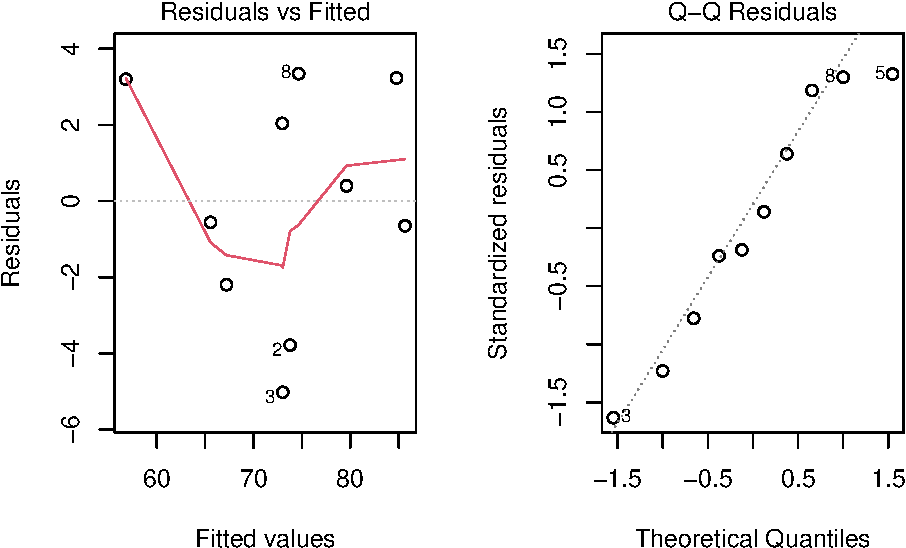
\includegraphics[keepaspectratio]{MultivariateStatisticalAnalysis_files/figure-latex/unnamed-chunk-7-1.pdf}}

\begin{center}\rule{0.5\linewidth}{0.5pt}\end{center}

\textbf{Ejercicio}: Supongamos que tenemos los siguientes datos: precio de vivienda según metros, habitaciones y distancia al centro.

Dataset

\begin{Shaded}
\begin{Highlighting}[]
\FunctionTok{set.seed}\NormalTok{(}\DecValTok{42}\NormalTok{)}
\NormalTok{n }\OtherTok{\textless{}{-}} \DecValTok{14}
\NormalTok{casas }\OtherTok{\textless{}{-}}\NormalTok{ tibble}\SpecialCharTok{::}\FunctionTok{tibble}\NormalTok{(}
  \AttributeTok{precio =} \FunctionTok{c}\NormalTok{(}\DecValTok{200}\NormalTok{,}\DecValTok{220}\NormalTok{,}\DecValTok{250}\NormalTok{,}\DecValTok{275}\NormalTok{,}\DecValTok{300}\NormalTok{,}\DecValTok{180}\NormalTok{,}\DecValTok{210}\NormalTok{,}\DecValTok{260}\NormalTok{,}\DecValTok{280}\NormalTok{,}\DecValTok{320}\NormalTok{,}\DecValTok{190}\NormalTok{,}\DecValTok{240}\NormalTok{,}\DecValTok{230}\NormalTok{,}\DecValTok{305}\NormalTok{),}
  \AttributeTok{metros =} \FunctionTok{c}\NormalTok{(}\DecValTok{80}\NormalTok{,}\DecValTok{90}\NormalTok{,}\DecValTok{100}\NormalTok{,}\DecValTok{110}\NormalTok{,}\DecValTok{120}\NormalTok{,}\DecValTok{70}\NormalTok{,}\DecValTok{85}\NormalTok{,}\DecValTok{105}\NormalTok{,}\DecValTok{115}\NormalTok{,}\DecValTok{130}\NormalTok{,}\DecValTok{75}\NormalTok{,}\DecValTok{95}\NormalTok{,}\DecValTok{92}\NormalTok{,}\DecValTok{125}\NormalTok{),}
  \AttributeTok{habitaciones =} \FunctionTok{c}\NormalTok{(}\DecValTok{2}\NormalTok{,}\DecValTok{3}\NormalTok{,}\DecValTok{3}\NormalTok{,}\DecValTok{4}\NormalTok{,}\DecValTok{4}\NormalTok{,}\DecValTok{2}\NormalTok{,}\DecValTok{3}\NormalTok{,}\DecValTok{3}\NormalTok{,}\DecValTok{4}\NormalTok{,}\DecValTok{5}\NormalTok{,}\DecValTok{2}\NormalTok{,}\DecValTok{3}\NormalTok{,}\DecValTok{3}\NormalTok{,}\DecValTok{4}\NormalTok{),}
  \AttributeTok{distancia\_centro =} \FunctionTok{c}\NormalTok{(}\DecValTok{5}\NormalTok{,}\DecValTok{4}\NormalTok{,}\DecValTok{6}\NormalTok{,}\DecValTok{3}\NormalTok{,}\DecValTok{2}\NormalTok{,}\DecValTok{8}\NormalTok{,}\DecValTok{6}\NormalTok{,}\DecValTok{3}\NormalTok{,}\DecValTok{2}\NormalTok{,}\DecValTok{1}\NormalTok{,}\DecValTok{7}\NormalTok{,}\DecValTok{5}\NormalTok{,}\DecValTok{4}\NormalTok{,}\DecValTok{2}\NormalTok{)}
\NormalTok{)}
\NormalTok{casas}
\end{Highlighting}
\end{Shaded}

\begin{verbatim}
## # A tibble: 14 x 4
##    precio metros habitaciones distancia_centro
##     <dbl>  <dbl>        <dbl>            <dbl>
##  1    200     80            2                5
##  2    220     90            3                4
##  3    250    100            3                6
##  4    275    110            4                3
##  5    300    120            4                2
##  6    180     70            2                8
##  7    210     85            3                6
##  8    260    105            3                3
##  9    280    115            4                2
## 10    320    130            5                1
## 11    190     75            2                7
## 12    240     95            3                5
## 13    230     92            3                4
## 14    305    125            4                2
\end{verbatim}

\begin{enumerate}
\def\labelenumi{\arabic{enumi})}
\tightlist
\item
  Ajusta \texttt{precio\ \textasciitilde{}\ metros} (simple) y \texttt{precio\ \textasciitilde{}\ metros\ +\ habitaciones\ +\ distancia\_centro} (múltiple).\\
\item
  Compara \(R^2\), \(R^2\) \textbf{ajustado} y \textbf{σ (RMSE)}.\\
\item
  Interpreta el coeficiente de \texttt{distancia\_centro}.\\
\item
  Revisa QQ-plot y residuales vs ajustados. ¿Algún patrón?
\end{enumerate}

Solución

\begin{Shaded}
\begin{Highlighting}[]
\NormalTok{m\_s }\OtherTok{\textless{}{-}} \FunctionTok{lm}\NormalTok{(precio }\SpecialCharTok{\textasciitilde{}}\NormalTok{ metros, }\AttributeTok{data=}\NormalTok{casas)}
\NormalTok{m\_m }\OtherTok{\textless{}{-}} \FunctionTok{lm}\NormalTok{(precio }\SpecialCharTok{\textasciitilde{}}\NormalTok{ metros }\SpecialCharTok{+}\NormalTok{ habitaciones }\SpecialCharTok{+}\NormalTok{ distancia\_centro, }\AttributeTok{data=}\NormalTok{casas)}

\NormalTok{broom}\SpecialCharTok{::}\FunctionTok{glance}\NormalTok{(m\_s)[,}\FunctionTok{c}\NormalTok{(}\StringTok{"r.squared"}\NormalTok{,}\StringTok{"adj.r.squared"}\NormalTok{)]}
\end{Highlighting}
\end{Shaded}

\begin{verbatim}
## # A tibble: 1 x 2
##   r.squared adj.r.squared
##       <dbl>         <dbl>
## 1     0.996         0.996
\end{verbatim}

\begin{Shaded}
\begin{Highlighting}[]
\NormalTok{broom}\SpecialCharTok{::}\FunctionTok{glance}\NormalTok{(m\_m)[,}\FunctionTok{c}\NormalTok{(}\StringTok{"r.squared"}\NormalTok{,}\StringTok{"adj.r.squared"}\NormalTok{)]}
\end{Highlighting}
\end{Shaded}

\begin{verbatim}
## # A tibble: 1 x 2
##   r.squared adj.r.squared
##       <dbl>         <dbl>
## 1     0.997         0.996
\end{verbatim}

\begin{Shaded}
\begin{Highlighting}[]
\NormalTok{broom}\SpecialCharTok{::}\FunctionTok{tidy}\NormalTok{(m\_m)}
\end{Highlighting}
\end{Shaded}

\begin{verbatim}
## # A tibble: 4 x 5
##   term             estimate std.error statistic      p.value
##   <chr>               <dbl>     <dbl>     <dbl>        <dbl>
## 1 (Intercept)        -8.67     14.9      -0.583 0.573       
## 2 metros              2.53      0.162    15.6   0.0000000236
## 3 habitaciones       -0.505     2.80     -0.180 0.861       
## 4 distancia_centro    1.38      0.974     1.42  0.187
\end{verbatim}

\begin{Shaded}
\begin{Highlighting}[]
\FunctionTok{par}\NormalTok{(}\AttributeTok{mfrow=}\FunctionTok{c}\NormalTok{(}\DecValTok{1}\NormalTok{,}\DecValTok{2}\NormalTok{))}
\FunctionTok{plot}\NormalTok{(m\_m, }\AttributeTok{which=}\DecValTok{1}\NormalTok{)}
\FunctionTok{plot}\NormalTok{(m\_m, }\AttributeTok{which=}\DecValTok{2}\NormalTok{)}
\end{Highlighting}
\end{Shaded}

\pandocbounded{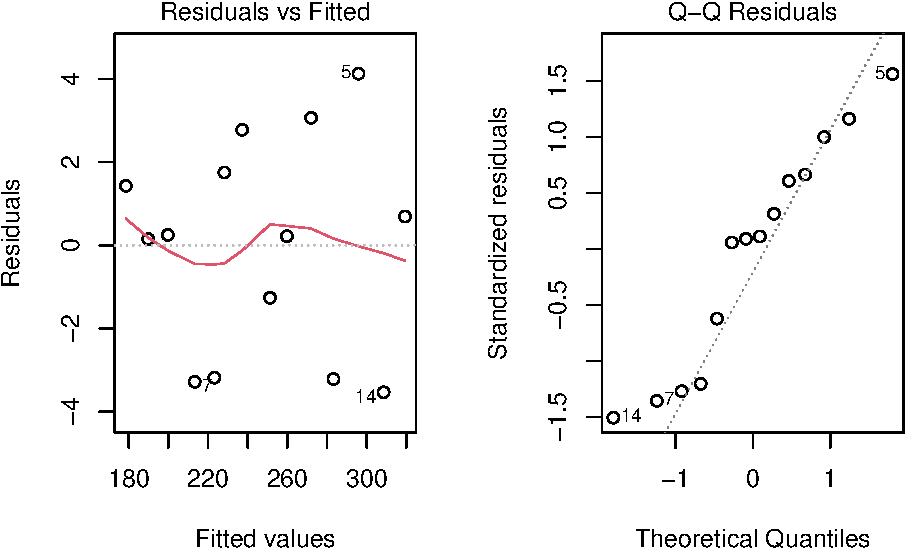
\includegraphics[keepaspectratio]{MultivariateStatisticalAnalysis_files/figure-latex/unnamed-chunk-9-1.pdf}}

\chapter{Análisis de Componentes Principales}\label{anuxe1lisis-de-componentes-principales}

\chapter{Análisis Factorial}\label{anuxe1lisis-factorial}

\chapter{Análisis de Conglomerados}\label{anuxe1lisis-de-conglomerados}

\chapter{Análisis de Discriminante}\label{anuxe1lisis-de-discriminante}

\chapter{Apéndices}\label{apuxe9ndices}

\section{Introducción a R}\label{introducciuxf3n-a-r}

\section{Git + Github}\label{git-github}

\section{Gráficas Multivariadas}\label{gruxe1ficas-multivariadas}

\section{Escalas de Medición}\label{escalas-de-mediciuxf3n}

\section{Valores Faltantes}\label{valores-faltantes}

  \bibliography{book.bib,packages.bib}

\end{document}
